En este capítulo, se presentan los cambios que se pueden generar para tener un programa mas fiel en su representación.
\section{Cambios que se deben realizar}
\begin{itemize}
    \item Mejorar modelos: Uno de los cambios mas fundamentales que se debe realizar para mejorar la experiencia e intentar lograr ser lo mas fiel posible en la representación del laboratorio.
    Se puede empezar por realizar un modelado fiel y a escala real de los objetos presentes en el laboratorio, para esto se presenta el programa que provee Intelitek para su brazo Scorbot ER-4U.
    En la Figura \ref{fig:modelo} se presenta la interfaz del programa RoboCell, el cual sirve para darle instrucciones al brazo robotico, ya sea real o simulado, en este ultimo se ve el detallado del modelo que da mejor sensación de realismo.
    \begin{figure}[h]
    \centering
    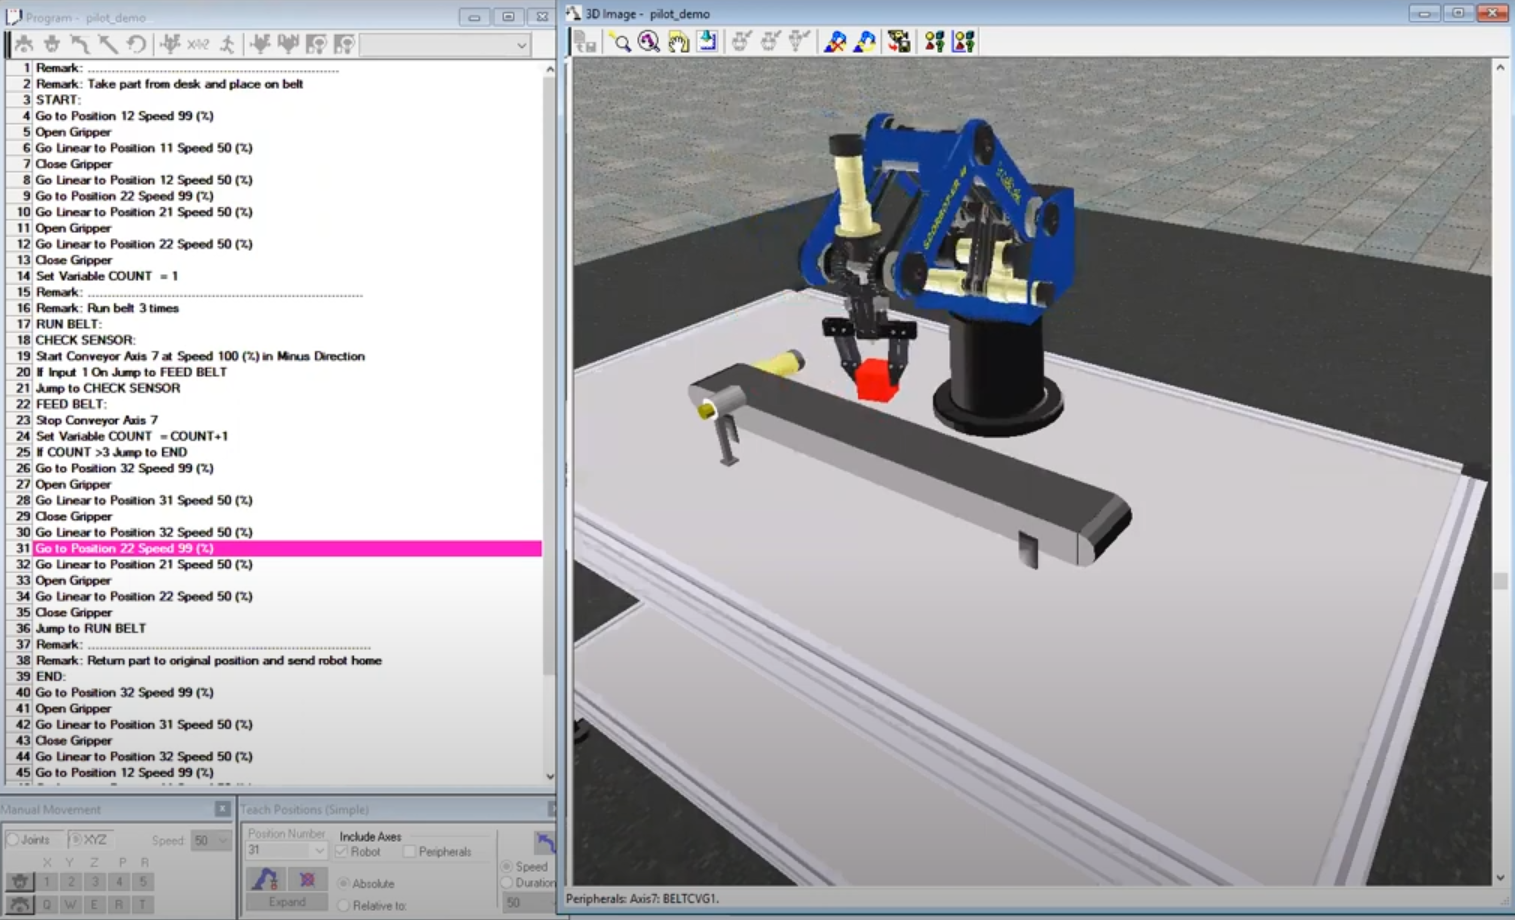
\includegraphics[height=5.82cm]{figures/modelo.png}
    \caption{Diseño interfaz: Módulo Principal}
    \label{fig:modelo}
    \end{figure}
    \item Opciones: Despliega las opciones de programa
\end{itemize}